\documentclass[conference]{IEEEtran}
\usepackage{tikz}
\IEEEoverridecommandlockouts
\usepackage{cite}
\usepackage{amsmath,amssymb,amsfonts}
\usepackage{algorithmic}
\usepackage{graphicx}
\usepackage{textcomp}
\usepackage{xcolor}
\usepackage{booktabs}
\usepackage{url}
\usepackage{iftex}
\ifXeTeX\usepackage{fontspec}\setmainfont{texgyretermes}[Extension=.otf,UprightFont=*-regular,BoldFont=*-bold,ItalicFont=*-italic,BoldItalicFont=*-bolditalic]\else\usepackage[T1]{fontenc}\fi
\graphicspath{{figures/}}
% let LaTeX place more floats per page so figures stay near their text
\renewcommand{\topfraction}{0.92}\renewcommand{\bottomfraction}{0.6}\renewcommand{\textfraction}{0.06}
\renewcommand{\floatpagefraction}{0.75}\renewcommand{\dbltopfraction}{0.92}\renewcommand{\dblfloatpagefraction}{0.75}
\setcounter{topnumber}{4}\setcounter{bottomnumber}{2}\setcounter{totalnumber}{6}\setcounter{dbltopnumber}{3}
% auto-generated by src/make_tables.py
\newcommand{\Rabnrec}{93.73}
\newcommand{\Raccalexnet}{87.58}
\newcommand{\Raccclassical}{77.25}
\newcommand{\Raccdensenet}{92.75}
\newcommand{\Raccefficientnetb}{91.58}
\newcommand{\Raccgooglenet}{89.92}
\newcommand{\Raccmobilenetv}{90.58}
\newcommand{\Raccresnet}{91.92}
\newcommand{\Raccvgg}{91.00}
\newcommand{\Raccvitb}{93.58}
\newcommand{\Rbestbase}{ViT-B/16}
\newcommand{\Rbestbaseacc}{93.58}
\newcommand{\Rbestbasemcc}{92.72}
\newcommand{\Rbypass}{25.3}
\newcommand{\Rcascpueighty}{15.7}
\newcommand{\Rcascpufps}{13.9}
\newcommand{\Rcascpums}{71.8}
\newcommand{\Rcascpuninety}{16.1}
\newcommand{\Rcasfps}{54}
\newcommand{\Rcasgmacs}{3.35}
\newcommand{\Rcasgmacseighty}{2.21}
\newcommand{\Rcasgmacsninety}{1.94}
\newcommand{\Rcasgpueighty}{69}
\newcommand{\Rcasgpuninety}{73}
\newcommand{\Rcasms}{18.6}
\newcommand{\Rcaspass}{74.7}
\newcommand{\Rcgastrovision}{20}
\newcommand{\Rckvasir}{8}
\newcommand{\Rcpufpsalexnet}{148.5}
\newcommand{\Rcpufpsdensenet}{27.2}
\newcommand{\Rcpufpsefficientnetb}{3.2}
\newcommand{\Rcpufpsgooglenet}{65.1}
\newcommand{\Rcpufpsmobilenetv}{19.8}
\newcommand{\Rcpufpsresnet}{37.0}
\newcommand{\Rcpufpsvgg}{13.3}
\newcommand{\Rcpufpsvitb}{12.5}
\newcommand{\Rcvcn}{612}
\newcommand{\Rcvcntotal}{612}
\newcommand{\Rcvcprop}{93.5}
\newcommand{\Rcvcproppolyp}{80.1}
\newcommand{\Rdropgastrovision}{7}
\newcommand{\Rdropkvasir}{0}
\newcommand{\Rfalexnet}{87.44}
\newcommand{\Rfclassical}{77.18}
\newcommand{\Rfdensenet}{92.73}
\newcommand{\Rfefficientnetb}{91.57}
\newcommand{\Rfgooglenet}{89.88}
\newcommand{\Rfmobilenetv}{90.56}
\newcommand{\Rfresnet}{91.89}
\newcommand{\Rfvgg}{90.92}
\newcommand{\Rfvitb}{93.56}
\newcommand{\Rfpsalexnet}{195}
\newcommand{\Rfpsdensenet}{40}
\newcommand{\Rfpsefficientnetb}{113}
\newcommand{\Rfpsgooglenet}{105}
\newcommand{\Rfpsmobilenetv}{127}
\newcommand{\Rfpsresnet}{54}
\newcommand{\Rfpsvgg}{31}
\newcommand{\Rfpsvitb}{51}
\newcommand{\Rgapbest}{1.7}
\newcommand{\Rgastrovisionacc}{78.15}
\newcommand{\Rgastrovisionbalacc}{67.55}
\newcommand{\Rgastrovisionbestbase}{ViT-B/16}
\newcommand{\Rgastrovisionbestbaseacc}{82.81}
\newcommand{\Rgastrovisionbestbasebacc}{66.29}
\newcommand{\Rgastrovisionf}{67.63}
\newcommand{\Rgastrovisionmcc}{75.63}
\newcommand{\Rgatecpums}{50.5}
\newcommand{\Rgatems}{7.9}
\newcommand{\Rgaterec}{99.3}
\newcommand{\Rgatespec}{66.4}
\newcommand{\Rgccvcarea}{8.5}
\newcommand{\Rgccvcpg}{65.0}
\newcommand{\Rgckvasirsegarea}{14.5}
\newcommand{\Rgckvasirsegpg}{81.2}
\newcommand{\Rgmacsalexnet}{0.71}
\newcommand{\Rgmacsdensenet}{2.83}
\newcommand{\Rgmacsefficientnetb}{0.38}
\newcommand{\Rgmacsgooglenet}{1.50}
\newcommand{\Rgmacsmobilenetv}{0.30}
\newcommand{\Rgmacsresnet}{4.09}
\newcommand{\Rgmacsvgg}{15.47}
\newcommand{\Rgmacsvitb}{11.27}
\newcommand{\Rkvasirsegn}{991}
\newcommand{\Rkvasirsegntotal}{1000}
\newcommand{\Rkvasirsegprop}{99.4}
\newcommand{\Rkvasirsegproppolyp}{98.5}
\newcommand{\Rmccalexnet}{85.95}
\newcommand{\Rmccclassical}{74.01}
\newcommand{\Rmccdensenet}{91.74}
\newcommand{\Rmccefficientnetb}{90.39}
\newcommand{\Rmccgooglenet}{88.51}
\newcommand{\Rmccmobilenetv}{89.27}
\newcommand{\Rmccresnet}{90.79}
\newcommand{\Rmccvgg}{89.74}
\newcommand{\Rmccvitb}{92.72}
\newcommand{\Rncvc}{612}
\newcommand{\Rngastrovision}{7,872}
\newcommand{\Rnkvasir}{8,000}
\newcommand{\Rnkvasirseg}{1,000}
\newcommand{\Rparamsalexnet}{57.0}
\newcommand{\Rparamsdensenet}{7.0}
\newcommand{\Rparamsefficientnetb}{4.0}
\newcommand{\Rparamsgooglenet}{5.6}
\newcommand{\Rparamsmobilenetv}{2.2}
\newcommand{\Rparamsresnet}{23.5}
\newcommand{\Rparamsvgg}{134.3}
\newcommand{\Rparamsvitb}{85.8}
\newcommand{\Rpropacc}{91.92}
\newcommand{\Rpropauc}{99.19}
\newcommand{\Rpropcihi}{93.4}
\newcommand{\Rpropcilo}{90.2}
\newcommand{\Rpropf}{91.89}
\newcommand{\Rpropkappa}{90.76}
\newcommand{\Rpropmcc}{90.79}
\newcommand{\Rpropprecision}{92.04}
\newcommand{\Rproprecall}{91.92}
\newcommand{\Rpropspecificity}{98.85}
\newcommand{\Rresnettransient}{54.2}
\newcommand{\Rressinglems}{18.6}
\newcommand{\Rrobbestbase}{ViT-B/16}
\newcommand{\Rrobbestbaseacc}{74.1}
\newcommand{\Rrobbestbasestream}{88.2}
\newcommand{\Rrobstream}{91.2}
\newcommand{\Rrobtransient}{91.8}
\newcommand{\Rsigbetter}{ViT-B/16}
\newcommand{\Rsigns}{VGG-16, ResNet-50, DenseNet-121, MobileNetV2, EfficientNet-B0}
\newcommand{\Rsigworse}{SIFT-BoVW+SVM, AlexNet, GoogLeNet}
\newcommand{\Rstagecpums}{28.5}
\newcommand{\Rstagems}{14.4}
\newcommand{\Rtau}{0.27}
\newcommand{\Rtaucur}{0.23}
  % every number quoted in the text (generated by src/make_tables.py)
\newcommand{\maybeinput}[1]{\IfFileExists{#1.tex}{\input{#1}}{\textbf{[\detokenize{#1} pending]}}}
\let\origincludegraphics\includegraphics
\renewcommand{\includegraphics}[2][]{\IfFileExists{figures/#2}{\origincludegraphics[#1]{#2}}{\fbox{\parbox{0.9\linewidth}{\centering figure \detokenize{#2} pending}}}}
\def\BibTeX{{\rm B\kern-.05em{\sc i\kern-.025em b}\kern-.08em
    T\kern-.1667em\lower.7ex\hbox{E}\kern-.125emX}}

\begin{document}

\title{Automated Gastric Cancer Diagnosis from Endoscopic Images}

\author{\IEEEauthorblockN{Nikhil Sanjay}
\IEEEauthorblockA{\textit{Department of Computer Science} \\
\textit{Amrita School of Computing}\\
Bengaluru, India \\
BL.EN.U4CSE23239}
\and
\IEEEauthorblockN{Andrew Tom Mathew}
\IEEEauthorblockA{\textit{Department of Computer Science} \\
\textit{Amrita School of Computing}\\
Bengaluru, India \\
BL.EN.U4CSE23269}
\and
\IEEEauthorblockN{Dr. Tripty Singh}
\IEEEauthorblockA{\textit{Department of Computer Science} \\
\textit{Amrita School of Computing,} \\
\textit{Bengaluru, India}
}
}

\maketitle

\begin{abstract}
Detection of gastrointestinal (GI) abnormalities in endoscopic images is a necessary step before targeted biopsy of
early-stage gastric ulcers and carcinomas. Although deep networks perform well on public benchmarks such as Kvasir,
real-world deployment is hindered by real-time constraints, strong class imbalance and transient camera artifacts that
cause false positives. This paper introduces a cascaded spatio-temporal framework: a lightweight MobileNetV2 gate
filters anatomically normal frames, so that a ResNet-50 feature extractor and a Bi-directional Long Short-Term Memory
(Bi-LSTM) network are run only on suspicious frames, where the Bi-LSTM verifies lesion stability across a sliding
window of $k=5$ frames. Focal loss handles class imbalance and Grad-CAM supplies visual explanations. The system is
benchmarked against a classical SIFT bag-of-visual-words + SVM pipeline and eight ImageNet-pretrained CNN/Transformer
baselines (AlexNet, VGG-16, GoogLeNet, ResNet-50, DenseNet-121, MobileNetV2, EfficientNet-B0, ViT-B/16) on
\emph{four} public databases (Kvasir v2, GastroVision, Kvasir-SEG, CVC-ClinicDB) using ten performance
evaluators. On Kvasir v2 the proposed cascade reaches \Rpropacc\% accuracy and an MCC of \Rpropmcc\%, \Rgapbest\ points
below the best single-frame baseline (\Rbestbase, \Rbestbaseacc\%). Its advantage appears on degraded frames: when the current
frame is hit by a transient artifact, it keeps \Rrobtransient\% accuracy versus \Rrobbestbaseacc\% for the most robust
single-frame baseline. The temporally smoothed gate passes \Rgaterec\% of abnormal frames while normal frames skip the
expensive stages, lowering the average cost to \Rcasgmacs\ GMACs per frame versus \Rgmacsresnet\ for ResNet-50.
\end{abstract}

\begin{IEEEkeywords}
Gastrointestinal cancer, endoscopy, computer-aided detection, deep learning, Bi-LSTM, focal loss, Grad-CAM, Kvasir.
\end{IEEEkeywords}

% =====================================================================
\section{Introduction \& Relevance}
\label{sec:introduction}

Malignancies of the gastrointestinal tract represent a considerable burden to world health. Their clinical outcome
depends heavily on the stage at which diagnosis occurs; screening for early-stage gastric ulcers and carcinomas is
therefore of particular importance to reduce mortality and avoid radical treatment. The clinical standard for GI
examination is endoscopy, which offers real-time, high-resolution visualisation of the mucosa of the oesophagus,
stomach and colon. However, detecting subtle, flat pre-cancerous lesions by eye limits the endoscopist's ability to
perform targeted biopsies in real time, as diagnostic performance depends heavily on skill and fatigue.

Traditional computer vision approaches based on hand-crafted descriptors such as SIFT \cite{lowe2004sift}, corner and
edge detectors often fail to robustly describe the homogeneous, highly specular textures of the GI tract.
Convolutional neural networks that learn hierarchical representations directly from pixels bypass the geometric and
photometric constraints of traditional image processing, and have become the dominant approach.

Automation should reduce the workload and fatigue of clinicians, but it must be designed around practical concerns:
false negatives cost lives, while false positives lead to unnecessary invasive biopsies and cost. The contributions of
this work are:
\begin{enumerate}
\item A three-stage \emph{cascaded spatio-temporal} pipeline (MobileNetV2 gate $\rightarrow$ ResNet-50 features
$\rightarrow$ Bi-LSTM) whose gate threshold is chosen to retain $\geq$99.5\% of abnormal frames while letting most
normal frames skip the expensive stages.
\item A synthetic video protocol that converts still-image databases into 5-frame clips with simulated camera motion
and four families of endoscopic artifacts, enabling a controlled study of temporal robustness.
\item A broad baseline comparison of nine methods on four public databases with ten performance evaluators, including
efficiency (parameters, GMACs, FPS), cross-database generalisation and quantitative Grad-CAM localisation.
\end{enumerate}

% =====================================================================
\section{Literature Review \& Core Research Gaps}
\label{sec:lit_review}

AI-based technologies in gastroenterology have been greatly facilitated by growth in computation, deep learning
methods and publicly available datasets. The Kvasir database \cite{pogorelov2017kvasir} was a milestone: a unified
multi-class benchmark spanning anatomical landmarks, pathological findings and endoscopic procedures, it accelerated
the design of computer-aided detection (CAD) systems. It was followed by larger collections such as HyperKvasir
\cite{borgli2020hyperkvasir} and GastroVision \cite{jha2023gastrovision}, and by pixel-annotated polyp sets such as
Kvasir-SEG \cite{jha2020kvasirseg} and CVC-ClinicDB \cite{bernal2015cvc}. Systematic reviews and meta-analyses have
provided convincing evidence for the superiority of CNNs over conventional machine learning for detecting gastric
cancer and colorectal lesions \cite{frontiers2026, wjg2025}.

\subsection{Architectural Evolution in Endoscopic Vision}
Early GI-lesion classifiers reused frameworks developed for natural images \cite{krizhevsky2012imagenet}. VGG
\cite{simonyan2014very} and Inception/GoogLeNet \cite{szegedy2015going, szegedy2016rethinking} improved multi-scale
feature extraction, but their parameter counts, memory requirements and slow inference constrain clinical use.
Residual connections in ResNet \cite{he2016deep} and dense feature concatenation in DenseNet \cite{huang2017densely}
enabled much deeper networks with better robustness on Kvasir \cite{mdpi2023sensors}; for example, ResNet-152 with
class activation mapping exceeded 93\% accuracy while localising discriminative regions
\cite{mdpi2023sensors, selvaraju2017grad}.

Beyond whole-image classification, U-Net \cite{ronneberger2015u} dominates lesion segmentation, while two-stage
detectors such as Faster R-CNN \cite{ren2015faster} and Mask R-CNN \cite{he2017mask} provide accurate box and
instance detection of polyps and ulcers, though often at the cost of processing speed.

\subsection{Real-Time Processing and Ensemble Techniques}
Because real-time feedback guides the endoscopist's instruments, efficient architectures such as MobileNetV2
\cite{sandler2018mobilenetv2} and EfficientNet \cite{tan2019efficientnet} use depthwise-separable convolutions and
compound scaling to deliver rich features at low cost. Hybrid ensembles inject global context from heavier networks
\cite{mdpi2024ensemble}, and single-stage detectors such as YOLOv4 \cite{bochkovskiy2020yolov4} remove the
region-proposal bottleneck. Optimising such models on skewed medical distributions requires the Adam family of
optimisers \cite{kingma2014adam, loshchilov2019adamw} and re-weighted losses such as Focal Loss \cite{lin2017focal}.
Vision Transformers \cite{dosovitskiy2020image} promise better global context but their cost and latency are a
concern for real-time endoscopy.

\subsection{Core Research Gaps}
Despite these advances, three gaps hinder the translation of static benchmark accuracy into dynamic clinical use:
\begin{enumerate}
\item \textbf{Throughput bottlenecks during live inference:} ensembles and Transformers achieve high accuracy on
static images, but their cost makes it hard to meet strict latency/FPS requirements.
\item \textbf{Class imbalance and under-represented rare pathologies:} cross-entropy is biased towards majority
classes (e.g.\ normal tissue); early flat pre-cancerous lesions remain under-represented in datasets such as Kvasir.
\item \textbf{Lack of clinical explainability:} high-accuracy classifiers seldom give fine-grained spatial
justification, and Grad-CAM heat-maps are rarely \emph{validated} against expert lesion annotations.
\end{enumerate}
In addition, almost all published systems classify frames independently and are thus vulnerable to transient
artifacts (motion blur, specular flashes, bubbles) that are ubiquitous in live video.

\subsection{Comparison with Baseline Architectures \& State-of-the-Art}
Table~\ref{tab:comparison} summarises the trade-offs reported in the literature, together with the results of the
proposed system measured in this work (Section~\ref{sec:results}).

\begin{table*}[t]
\caption{Performance trade-offs of endoscopic image analysis approaches (literature values are typical figures reported on Kvasir-type data; the last row is measured in this work).}
\label{tab:comparison}
\centering
\begin{tabular}{lllcc}
\toprule
\textbf{Reference Framework} & \textbf{Analysis Modality} & \textbf{Primary Optimization Focus} & \textbf{Typical Accuracy} & \textbf{Real-Time Efficiency} \\ \midrule
VGG-16 / Inception \cite{simonyan2014very, szegedy2016rethinking} & Static image & Multi-scale feature extraction & $\sim$85--88\% & Low FPS \\
ResNet-152 + CAM \cite{mdpi2023sensors} & Static image & Discriminative lesion localisation & $>$93\% & Medium FPS \\
MobileNetV2 / EfficientNet \cite{sandler2018mobilenetv2, tan2019efficientnet} & Static image & High-throughput processing & $\sim$90\% & High FPS \\
YOLOv4 \cite{bochkovskiy2020yolov4} & Static detection & Rapid bounding-box generation & $\sim$91\% & Very high FPS \\
\textbf{Proposed system} & \textbf{Spatio-temporal} & \textbf{Gated sequential lesion tracking} & \textbf{\Rpropacc\%} & \textbf{\Rcasgmacs\ GMACs/frame} \\ \bottomrule
\end{tabular}
\end{table*}

% =====================================================================
\section{Databases and Materials}
\label{sec:dataset}

Four public databases are used (Table~\ref{tab:datasets}, Fig.~\ref{fig:datasets}). \textbf{Kvasir v2}
\cite{pogorelov2017kvasir} is the primary benchmark: 8,000 expert-annotated images, balanced across eight classes of
anatomical landmarks (Z-line, pylorus, cecum), pathological findings (oesophagitis, polyps, ulcerative colitis) and
procedures (dyed-lifted polyps, dyed resection margins). \textbf{GastroVision} \cite{jha2023gastrovision} is a strongly imbalanced multi-class database
covering the upper and lower GI tract, including gastric findings such as gastric polyps, ulcers, erythema and
colorectal cancer. Classes with fewer than 30 images (\Rdropgastrovision\ in GastroVision) are removed, because they cannot be split into train/validation/test.
\textbf{Kvasir-SEG} \cite{jha2020kvasirseg} and \textbf{CVC-ClinicDB} \cite{bernal2015cvc} contain polyp frames with
pixel-level expert masks; they are never used for training and serve as external test sets for cross-database
generalisation and quantitative Grad-CAM localisation. CVC-ClinicDB was acquired with a different endoscope at a
different hospital, making it a genuine domain-shift test.

Each classification database is split once, stratified by class, into 70/15/15\% train/validation/test sets (seed
42). Raw images (720$\times$576 to 1920$\times$1072 pixels) are resized with bicubic interpolation to
224$\times$224$\times$3 and cached as 8-bit tensors, so high-resolution JPEGs are decoded only once.

\maybeinput{tables/datasets}

\begin{figure*}[t]
\centering
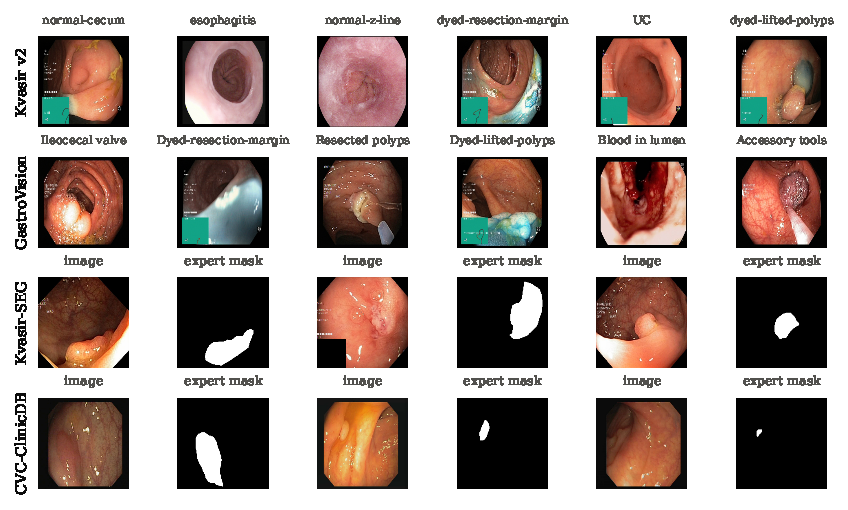
\includegraphics[width=\textwidth]{fig_datasets.pdf}
\caption{Samples from the four databases: random classes from Kvasir v2 and GastroVision, and image/mask
pairs from the two external polyp databases.}
\label{fig:datasets}
\end{figure*}

The pipeline is implemented in PyTorch 2 with torchvision ImageNet weights and runs on an Apple M5 GPU (Metal/MPS
backend) with mixed-precision (FP16) arithmetic; augmentation, artifact simulation and clip synthesis are executed on
the GPU to avoid data-loading bottlenecks. All code, configuration and logs are released with the paper.

% =====================================================================
\section{Proposed System Design}
\label{sec:system_design}

Considering the clinical constraints of high-throughput endoscopy and the imbalanced nature of GI disease, the system
is designed as a cascaded, spatio-temporal diagnosis pipeline (Fig.~\ref{fig:architecture}).

\subsection{Synthetic Clips from Still Images}
To emulate the time-series nature of clinical video from still-image databases, each image $I$ is turned into a
$k=5$-frame clip $\{I_{t-4},\dots,I_t\}$ by a smooth simulated camera trajectory: a per-clip random velocity in
rotation ($\le$4$^\circ$/frame), zoom ($\le$3\%/frame) and translation ($\le$3\%/frame) is integrated backwards from
the current frame $I_t$. Any frame may then be replaced by a corrupted version produced by one of four artifact
models (Fig.~\ref{fig:artifacts}): \emph{motion blur} (random line kernel, 11--23 px), \emph{defocus} (Gaussian,
$\sigma\in[2.5,6]$), \emph{specular flash} (global over-exposure plus saturated specular blobs) and
\emph{noise/occlusion} (Gaussian sensor noise and a dark occluding region, e.g.\ a bubble or debris).

\begin{figure}[t]
\centering
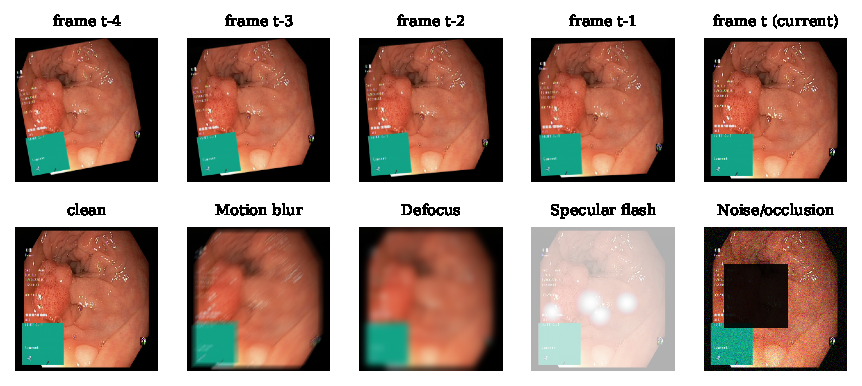
\includegraphics[width=\linewidth]{fig_artifacts.pdf}
\caption{Top: a synthetic 5-frame clip generated from one Kvasir polyp image. Bottom: the four simulated artifact
families applied to the current frame.}
\label{fig:artifacts}
\end{figure}

\subsection{Spatio-Temporal Architectural Flow}
\begin{figure}[t]
\centering
\resizebox{\linewidth}{!}{%
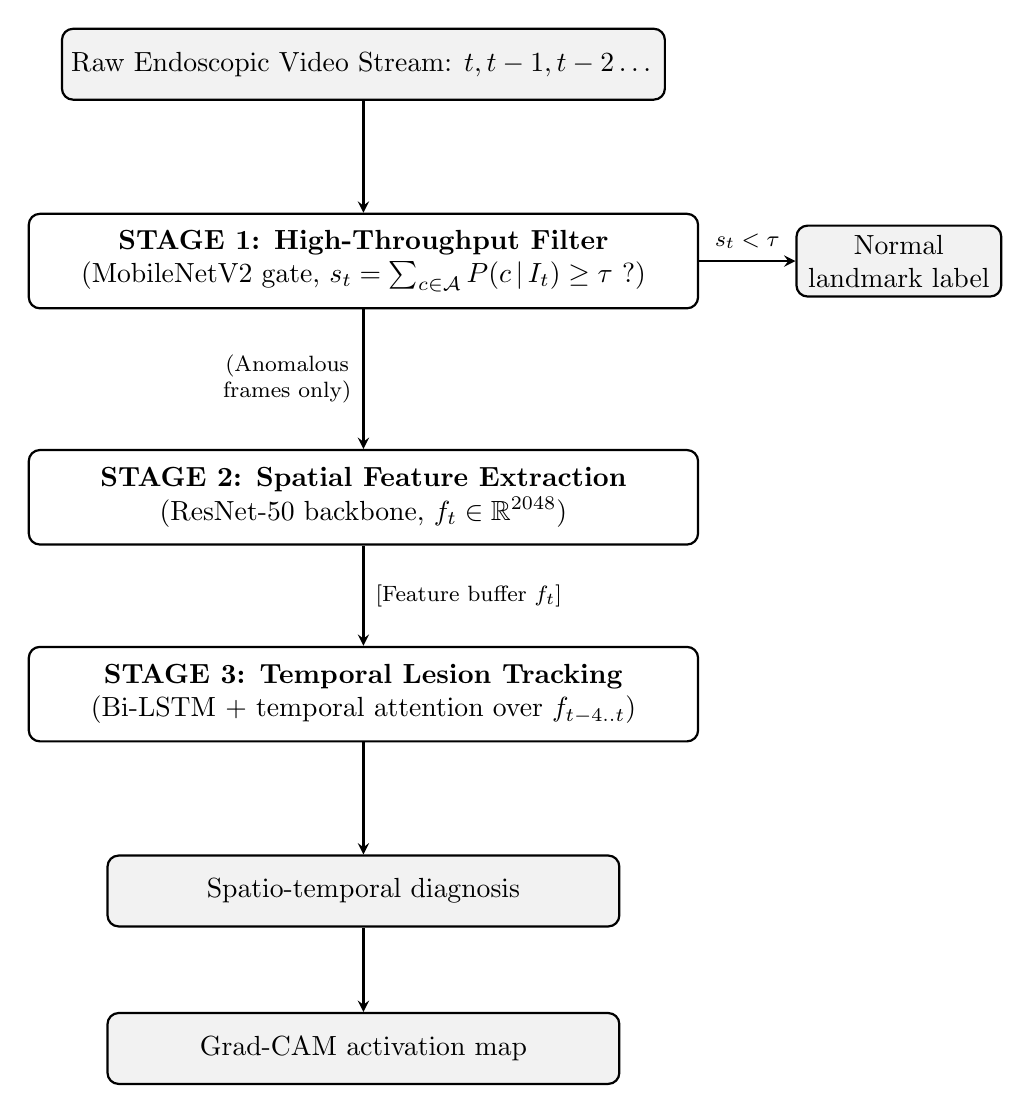
\begin{tikzpicture}[
    >=stealth, node distance=2.5cm,
    mainbox/.style={rectangle, rounded corners=4pt, draw, thick, minimum width=8.5cm, minimum height=1.2cm, align=center, fill=white},
    iobox/.style={rectangle, rounded corners=4pt, draw, thick, minimum width=6.5cm, minimum height=0.9cm, align=center, fill=gray!10},
    arrowlabel/.style={font=\footnotesize, align=center, inner sep=4pt}]
\node[iobox] (input) {Raw Endoscopic Video Stream: $t, t-1, t-2\dots$};
\node[mainbox, below of=input] (stage1) {\textbf{STAGE 1: High-Throughput Filter}\\(MobileNetV2 gate, $s_t=\sum_{c\in\mathcal{A}}P(c\,|\,I_t)\ge\tau$ ?)};
\node[mainbox, below of=stage1, yshift=-0.5cm] (stage2) {\textbf{STAGE 2: Spatial Feature Extraction}\\(ResNet-50 backbone, $f_t\in\mathbb{R}^{2048}$)};
\node[mainbox, below of=stage2] (stage3) {\textbf{STAGE 3: Temporal Lesion Tracking}\\(Bi-LSTM + temporal attention over $f_{t-4..t}$)};
\node[iobox, below of=stage3] (spatio) {Spatio-temporal diagnosis};
\node[iobox, below of=spatio, yshift=0.5cm] (gradcam) {Grad-CAM activation map};
\node[iobox, right of=stage1, xshift=4.3cm, minimum width=2.6cm] (normal) {Normal\\landmark label};
\draw[->, thick] (input) -- (stage1);
\draw[->, thick] (stage1) -- node[left, arrowlabel] {(Anomalous\\frames only)} (stage2);
\draw[->, thick] (stage1) -- node[above, arrowlabel] {$s_t<\tau$} (normal);
\draw[->, thick] (stage2) -- node[right, arrowlabel] {[Feature buffer $f_t$]} (stage3);
\draw[->, thick] (stage3) -- (spatio);
\draw[->, thick] (spatio) -- (gradcam);
\end{tikzpicture}}
\caption{Proposed spatio-temporal cascaded architecture. Frames whose abnormality score $s_t$ is below $\tau$ exit
after Stage 1 with a normal-landmark label.}
\label{fig:architecture}
\end{figure}

\textbf{Stage 1 -- gate.} A MobileNetV2 classifier is trained over all classes; its binary gate score is the total
probability of the abnormal classes $\mathcal{A}$ (pathology and interventions), $s_t=\sum_{c\in\mathcal{A}}
P(c\,|\,I_t)$. Its efficiency comes from depthwise-separable convolution, which factorises a standard convolution into
a depthwise spatial convolution and a $1\times1$ pointwise convolution. For an input feature map $F$ and depthwise
kernel $\hat{K}$, the depthwise output is
\begin{equation}
    \hat{G}_{k,l,m} = \sum_{i,j} \hat{K}_{i,j,m} \cdot F_{k+i-1, l+j-1, m},
\end{equation}
followed by a pointwise linear combination with a $1 \times 1$ kernel $P$:
\begin{equation}
    G_{k,l,n} = \sum_{m} P_{m,n} \cdot \hat{G}_{k,l,m}.
\end{equation}
Frames with $s_t<\tau$ are labelled with the gate's most probable \emph{normal} class and skip the deeper stages,
which reduces the average latency.

\textbf{Stage 2 -- spatial features.} Frames with $s_t\ge\tau$ are passed to a ResNet-50 whose global-pooled
output is a 2048-d spatial feature vector $f_t$, pushed into a first-in-first-out buffer of the last $k$ features.

\textbf{Stage 3 -- temporal verification.} To suppress false positives caused by transient blur or light flashes, a
Bi-LSTM \cite{hochreiter1997lstm, schuster1997bidirectional} processes the buffer. After a LayerNorm-and-linear
projection to 512-d, it computes forward and backward hidden states (256 units each) at every time step:
\begin{equation}
\begin{aligned}
    \overrightarrow{h}_t &= \text{LSTM}_{fwd}(f_t, \overrightarrow{h}_{t-1}),\\
    \overleftarrow{h}_t &= \text{LSTM}_{bwd}(f_t, \overleftarrow{h}_{t+1}),\\
    a_t &= \operatorname{softmax}_t\big(w_a^\top[\overrightarrow{h}_t \oplus \overleftarrow{h}_t]\big),\\
    y &= W_y \textstyle\sum_t a_t[\overrightarrow{h}_t \oplus \overleftarrow{h}_t] + b_y,
\end{aligned}
\end{equation}
where $\oplus$ is concatenation, $a_t$ is a learned temporal attention weight that lets the network down-weight
corrupted frames, and $W_y, b_y$ are the parameters of the output layer.

% =====================================================================
\section{Implementation}
\label{sec:implementation}

\subsection{Phase 1: Data Ingestion}
A preprocessing script indexes each database, performs the stratified split and caches the resized images as NumPy
arrays. The full training set is held in memory and mini-batches are moved to the GPU, where a stochastic
augmentation policy is applied per sample (horizontal/vertical flips, rotation $\pm20^\circ$, zoom $\pm12$\%,
shift $\pm8$\%, brightness/contrast/saturation jitter $\pm20$\%).

\subsection{Phase 2: Training the Spatial Stages}
The Stage-1 MobileNetV2 and the Stage-2 ResNet-50 are initialised from ImageNet and fine-tuned end-to-end with the
Focal Loss
\begin{equation}
    \text{FL}(p_t) = -\alpha_t (1 - p_t)^\gamma \log(p_t),
\end{equation}
where $p_t$ is the predicted probability of the ground-truth class, $\gamma=2$ down-weights easy examples and
$\alpha_t$ is a tempered inverse-frequency class weight ($\alpha_c\propto 1/\sqrt{n_c}$, normalised to mean 1). The
loss is computed from log-softmax outputs for numerical stability. Optimisation uses AdamW
\cite{loshchilov2019adamw} (weight decay $10^{-2}$, decoupled from the gradient update), batch size 32 and a
\emph{differential learning rate}: $10^{-4}$ for the pretrained backbone and $10^{-3}$ for the new classifier head, to
avoid catastrophic forgetting of ImageNet features. The learning rate follows a cosine annealing schedule
\cite{loshchilov2017sgdr} after a 10\% linear warm-up:
\begin{equation}
    \eta_t = \eta_{min} + \frac{1}{2}(\eta_{max} - \eta_{min})\left(1 + \cos\left(\frac{T_{cur}}{T_{max}}\pi\right)\right),
\end{equation}
where $T_{cur}$ is the current step and $T_{max}$ the total number of steps. Because ImageNet-pretrained networks
converge quickly on these data (Fig.~\ref{fig:curves}), training runs for 5 epochs on Kvasir and 4 epochs on
GastroVision; the checkpoint with the best validation macro-F1 is kept.

\subsection{Phase 3: Training the Temporal Stage}
With Stages 1--2 frozen, three synthetic clips (one on GastroVision, to save time) are generated for every training image (with augmentation, and each
frame corrupted with probability 0.3), and their ResNet-50 features are cached. The Bi-LSTM is trained on these
features for 40 epochs with focal loss, AdamW (lr $10^{-3}$, cosine annealing) and random temporal reversal. Model
selection uses an equal mix of clean and artifact-corrupted validation clips. Decoupling the expensive CNN from the
recurrent model in this way reduces the temporal-training cost from hours to seconds.

\textbf{Gate threshold.} Missing a lesion is far more costly than running Stage 2 unnecessarily, so $\tau$ is chosen
on the validation set as the \emph{largest} threshold for which the gate still passes $\ge$99.5\% of abnormal frames
(Fig.~\ref{fig:tau}). This gives $\tau=\Rtau$ on Kvasir.

\subsection{Phase 4: Evaluation and Explainability}
\textbf{Grad-CAM.} The heat-map is computed from the gradients flowing into the last convolutional block of the
Stage-2 ResNet-50 \cite{selvaraju2017grad}. The importance weight of feature map $A^k$ for class $c$ is
\begin{equation}
    \alpha_k^c = \frac{1}{Z} \sum_i \sum_j \frac{\partial y^c}{\partial A_{ij}^k},
\end{equation}
and the weighted maps are combined and rectified so that only positively contributing features remain:
\begin{equation}
    L_{\text{Grad-CAM}}^c = \text{ReLU} \left( \sum_k \alpha_k^c A^k \right).
\end{equation}
For display, $L^c$ is up-sampled to the input resolution, normalised and scaled by the model's confidence for class
$c$ before being overlaid on the frame.

% =====================================================================
\section{Experimental Setup}
\label{sec:setup}

\subsection{Baselines}
Nine baselines are compared with the proposed system: (i) a \textbf{classical} pipeline of dense SIFT
\cite{lowe2004sift} descriptors quantised into a 256-word bag of visual words \cite{csurka2004bovw}, concatenated with
an HSV colour histogram and a uniform LBP texture histogram \cite{ojala2002lbp}, classified by an RBF-kernel SVM
\cite{cortes1995svm}; and (ii) eight ImageNet-pretrained deep networks fine-tuned with the \emph{same} data,
augmentation, optimiser, schedule and epoch budget as the proposed stages but with standard cross-entropy: AlexNet
\cite{krizhevsky2012imagenet}, VGG-16 (with batch normalisation) \cite{simonyan2014very}, GoogLeNet
\cite{szegedy2015going}, ResNet-50 \cite{he2016deep}, DenseNet-121 \cite{huang2017densely}, MobileNetV2
\cite{sandler2018mobilenetv2}, EfficientNet-B0 \cite{tan2019efficientnet} and ViT-B/16 \cite{dosovitskiy2020image}.

\subsection{Performance Evaluators}
With $TP, TN, FP, FN$ computed per class (one-vs-rest) and macro-averaged, we report: Accuracy;
Precision $=TP/(TP+FP)$; Recall (sensitivity) $=TP/(TP+FN)$; F1 $=2PR/(P+R)$; Specificity $=TN/(TN+FP)$; balanced
accuracy (mean per-class recall); the area under the one-vs-rest ROC curve (AUC); Cohen's $\kappa$; and the Matthews
Correlation Coefficient, which remains informative under class imbalance \cite{chicco2020mcc}:
\begin{equation}
    \text{MCC} = \frac{TP \cdot TN - FP \cdot FN}{\sqrt{D}},
\end{equation}
where $D = (TP+FP)(TP+FN)(TN+FP)(TN+FN)$; for $K>2$ classes the multi-class generalisation computed from the full
confusion matrix is used. Efficiency is measured by parameter count, GMACs per frame and batch-1 throughput (FPS) on
the GPU after warm-up. Explainability is quantified against expert masks by the pointing-game hit rate
\cite{zhang2018pointing}, the fraction of CAM energy inside the mask and the IoU of the CAM thresholded at 0.5.

\subsection{Test Protocols}
\emph{Clean}: the current frame is the unmodified test image (single-frame baselines see exactly the standard test
set; the proposed system additionally sees four preceding synthetic frames). \emph{Transient artifact}: only the
current frame is corrupted with one of the four artifact types. \emph{Artifact stream}: every frame of the clip is
independently corrupted with probability 0.3. \emph{Cross-database}: Kvasir-trained models are applied unchanged to
Kvasir-SEG and CVC-ClinicDB.

% =====================================================================
\section{Results and Discussion}
\label{sec:results}
% Auto-generated numbers come from tables/macros.tex (src/make_tables.py).

\subsection{Baseline Comparison on Kvasir v2}
Table~\ref{tab:main} compares all methods on the Kvasir v2 test set with eight classification evaluators and
three efficiency evaluators; Fig.~\ref{fig:bars} visualises accuracy, macro-F1 and MCC on both classification
databases. The hand-crafted SIFT-BoVW+SVM pipeline reaches \Raccclassical\% accuracy, confirming that
learned features are far better suited to the homogeneous, specular GI mucosa. Among the deep baselines, accuracy
ranges from \Raccalexnet\% (AlexNet) to \Rbestbaseacc\% (\Rbestbase). The proposed cascade reaches \Rpropacc\%
accuracy, \Rpropf\% macro-F1, \Rpropmcc\% MCC and \Rpropauc\% AUC. On clean, curated still images it is
therefore \Rgapbest\ points below the best single-frame network and level with its own ResNet-50 backbone
(\Raccresnet\%); this is expected, since the temporal stage cannot add information when every frame is clean and the
neighbouring frames are near-duplicates. The value of the design lies elsewhere: it is the only model that remains
accurate when frames are degraded (Section~\ref{sec:robust}), and a stronger backbone (e.g.\ ViT-B/16 or
DenseNet-121) could be dropped into Stage 2 without changing the rest of the pipeline. The training curves in Fig.~\ref{fig:curves} show that every pretrained
network converges within the 5-epoch budget, so the comparison is not biased by under-training.

\maybeinput{tables/main_kvasir}

Because the test sets contain about 1,200--1,600 images, accuracy differences of one or two points are within
sampling noise. Table~\ref{tab:stats} therefore reports bootstrap 95\% confidence intervals and exact McNemar tests
against the proposed system. On Kvasir the proposed cascade (\Rpropacc\%, CI \Rpropcilo--\Rpropcihi\%) is
significantly better than \Rsigworse, statistically indistinguishable from \Rsigns, and significantly behind only
\Rsigbetter.

\maybeinput{tables/stats}

\begin{figure*}[t]
\centering
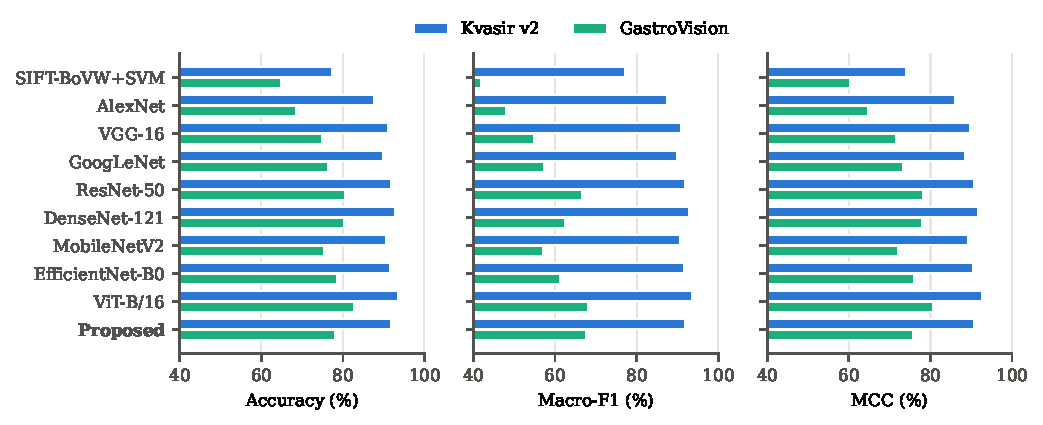
\includegraphics[width=\textwidth]{fig_baseline_comparison.pdf}
\caption{Baseline comparison on the two classification databases (test sets). The proposed system is the
bottom row of each panel.}
\label{fig:bars}
\end{figure*}

\begin{figure*}[t]
\centering
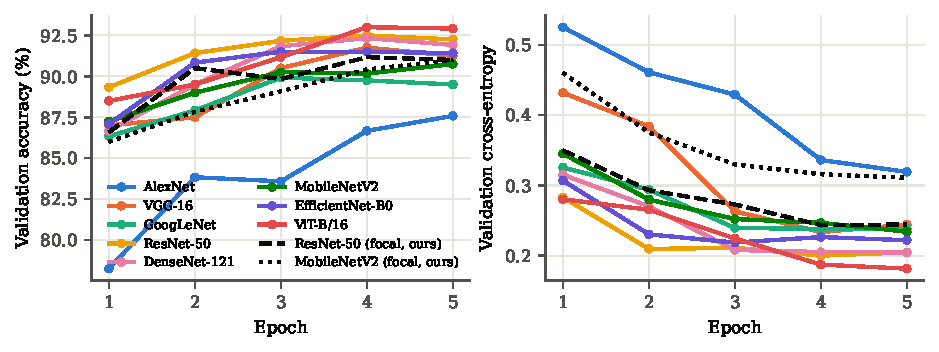
\includegraphics[width=\textwidth]{fig_training_curves.pdf}
\caption{Validation accuracy and cross-entropy per epoch on Kvasir v2 for all deep baselines and for the two
focal-loss stages of the proposed system (black).}
\label{fig:curves}
\end{figure*}

The confusion matrices (Fig.~\ref{fig:confusion}) show that the dominant error on Kvasir is the confusion between
\emph{oesophagitis} and the \emph{normal Z-line}, and between \emph{dyed-lifted polyps} and \emph{dyed resection
margins}. Both pairs are visually near-identical and are known to be ambiguous even for annotators, which is also
visible in the per-class F1 scores (Fig.~\ref{fig:perclass}). The ROC curves (Fig.~\ref{fig:roc}) show
micro-averaged AUCs above 0.99 for all deep models on Kvasir.

\begin{figure*}[t]
\centering
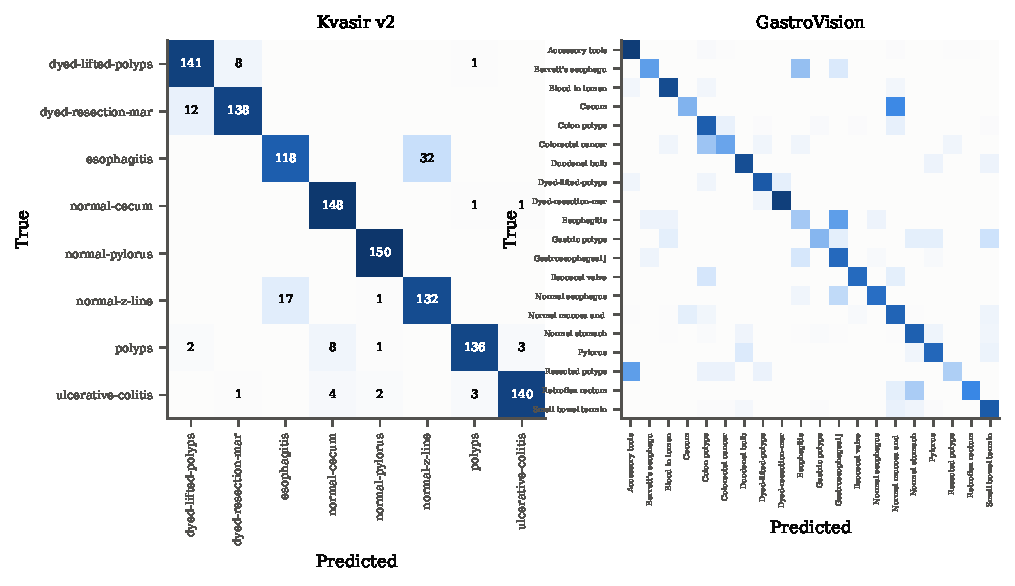
\includegraphics[width=\textwidth]{fig_confusion.pdf}
\caption{Confusion matrices of the proposed cascade on the clean test sets (rows: true class).}
\label{fig:confusion}
\end{figure*}

\begin{figure*}[t]
\centering
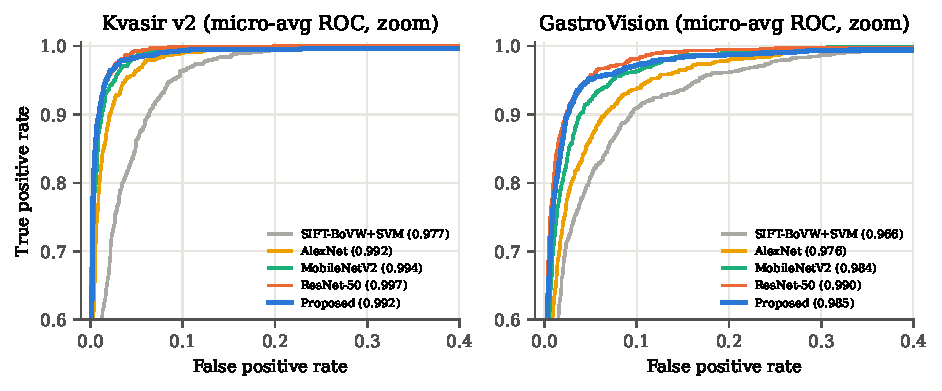
\includegraphics[width=\textwidth]{fig_roc.pdf}
\caption{Micro-averaged ROC curves (zoomed into the upper-left corner) with AUC in brackets.}
\label{fig:roc}
\end{figure*}

\begin{figure}[t]
\centering
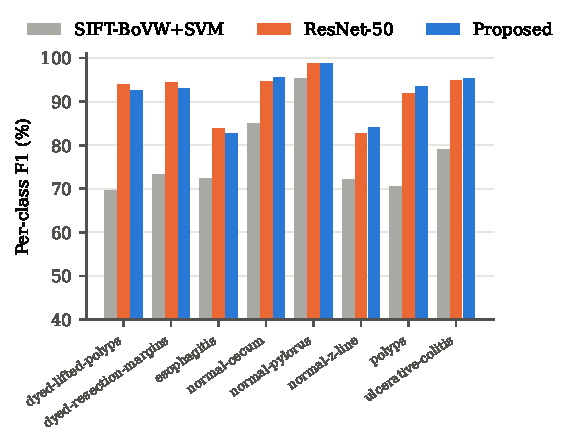
\includegraphics[width=\linewidth]{fig_perclass_f1.pdf}
\caption{Per-class F1 on Kvasir v2.}
\label{fig:perclass}
\end{figure}

\subsection{Generalisation to a Second Classification Database}
Table~\ref{tab:multidb} repeats the comparison on GastroVision, which covers more classes (including gastric
findings) and is strongly imbalanced. Here plain accuracy is dominated by the large classes, so balanced accuracy and
MCC are the more informative evaluators. The proposed cascade obtains \Rgastrovisionacc\% accuracy and
\Rgastrovisionbalacc\% balanced accuracy (best baseline: \Rgastrovisionbestbase, \Rgastrovisionbestbaseacc\% /
\Rgastrovisionbestbasebacc\%). The classical baseline collapses on this database, especially in balanced accuracy,
because its fixed descriptors cannot separate the many fine-grained classes. Although its plain accuracy is lower than that of the
strongest single-frame networks, the proposed cascade has the highest balanced accuracy of all methods, i.e.\ the best
recall on the rare classes, which is the intended effect of the focal loss and the abnormality-oriented gate.

\maybeinput{tables/multi_db}

\subsection{Robustness to Endoscopic Artifacts}
\label{sec:robust}
Table~\ref{tab:robust} and Fig.~\ref{fig:robust} report Kvasir accuracy when the current frame is hit by a
transient artifact. Every single-frame model degrades sharply, because it has nothing to classify except the
corrupted frame: averaged over the four artifact types, the most robust baseline (\Rrobbestbase) keeps only
\Rrobbestbaseacc\%, and ResNet-50 keeps \Rresnettransient\%. The proposed system keeps \Rrobtransient\%, essentially
its clean accuracy, and \Rrobstream\% on a random artifact stream where 30\% of all frames are corrupted. This is the
behaviour the temporal stage was designed for: a lesion that is visible in the preceding frames is not lost because of
one blurred or flashed frame, and an artifact cannot create a lesion that the preceding frames do not show.

\maybeinput{tables/robustness}

\begin{figure*}[t]
\centering
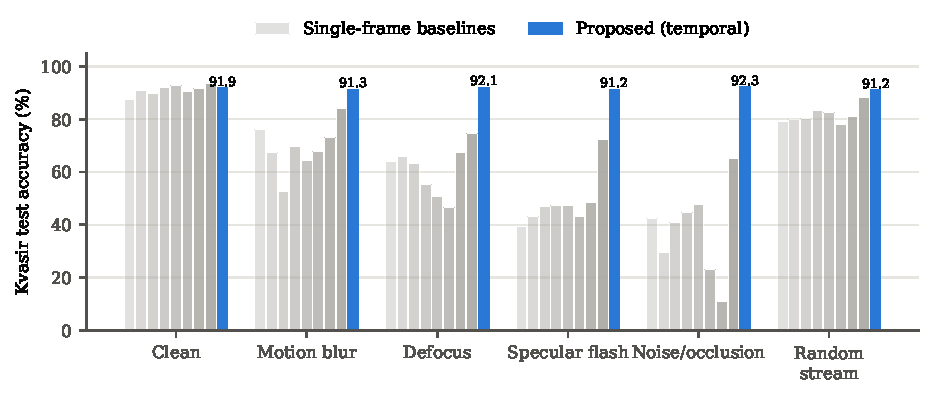
\includegraphics[width=\textwidth]{fig_robustness.pdf}
\caption{Kvasir test accuracy under transient artifacts on the current frame and on a random artifact stream.
Grey bars: the eight single-frame deep baselines (left to right as in Table~\ref{tab:main}); blue: proposed.}
\label{fig:robust}
\end{figure*}

Fig.~\ref{fig:attention} shows why: the learned temporal attention $a_t$ assigns corrupted frames an average weight
an order of magnitude lower than clean frames at every position of the window, i.e.\ the Bi-LSTM has learned
\emph{which} frames to trust without any frame-quality supervision.

\begin{figure}[t]
\centering
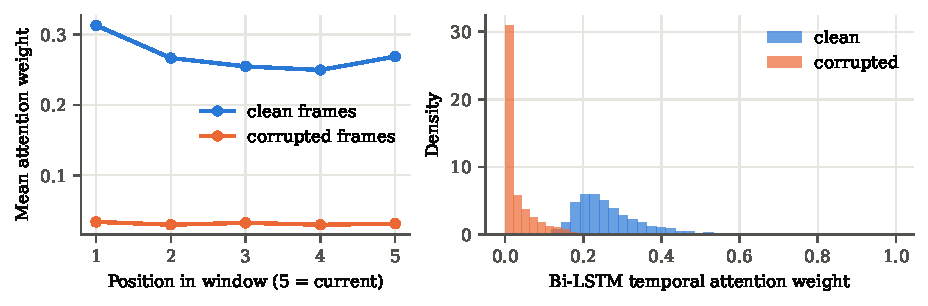
\includegraphics[width=\linewidth]{fig_attention.pdf}
\caption{Bi-LSTM temporal attention on the artifact stream: mean weight per window position (left) and the
distribution of weights (right) for clean versus corrupted frames.}
\label{fig:attention}
\end{figure}

\subsection{Ablation Study}
Table~\ref{tab:ablation} isolates each component. (i) Replacing cross-entropy by focal loss changes clean Kvasir
accuracy only marginally on this balanced database. (ii) Any form of temporal aggregation removes most of the artifact
sensitivity of the single-frame model. Simple mean pooling of the per-frame probabilities is a strong baseline on our
synthetic clips, because neighbouring frames are near-duplicates; the Bi-LSTM performs comparably while additionally
providing interpretable attention weights and the capacity to model genuine appearance changes in real video.
(iii) Routing on the \emph{current} frame only makes the gate itself the weak point: a flash or a dark occlusion can
push a lesion frame below $\tau$ and cause a bypass. Averaging the gate probabilities over the five-frame buffer
(gate scores are computed once per frame anyway) removes this failure mode at no extra cost, and the full cascade
matches the un-gated temporal model while skipping Stages 2--3 for part of the stream.

\maybeinput{tables/ablation}

\subsection{Computational Efficiency and the Stage-1 Gate}
The gate threshold is selected on validation data as the largest $\tau$ that keeps the abnormal-frame recall at
$\ge$99.5\% (Fig.~\ref{fig:tau}); this gives $\tau=\Rtau$ on Kvasir, a test-set gate recall of \Rgaterec\% for
abnormal frames and a bypass rate of \Rbypass\% of all frames (Table~\ref{tab:gate}). Measured on the idle M5 GPU at
batch size 1, the gate costs \Rgatems~ms and Stages 2--3 cost \Rstagems~ms per frame, so the expected cost of the
cascade at Kvasir's class mix is \Rcasms~ms (\Rcasfps~FPS) and \Rcasgmacs~GMACs, against \Rressinglems~ms and
\Rgmacsresnet~GMACs for ResNet-50 on every frame: at this prevalence the cascade roughly breaks even, while adding the
temporal verification for free. On the CPU, PyTorch's depthwise-convolution kernels for this ARM processor are
inefficient (MobileNetV2 is slower than ResNet-50 despite needing 13$\times$ fewer MACs), so the gate brings no CPU
wall-clock gain without an optimised mobile runtime; CPU figures are nevertheless reported in Table~\ref{tab:main}.

\begin{figure}[t]
\centering
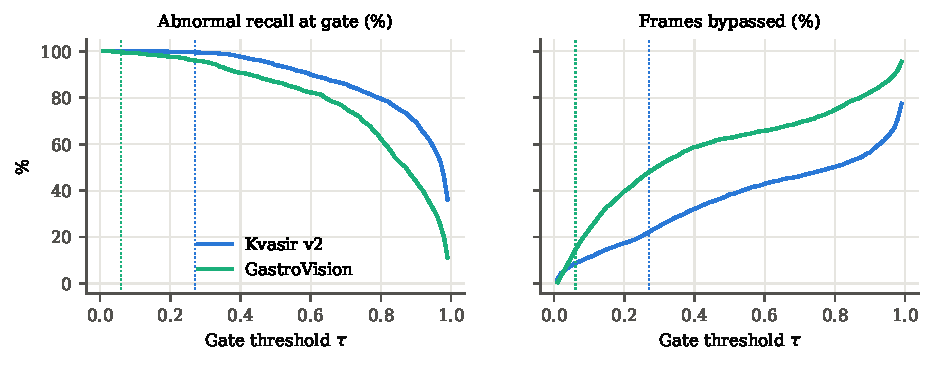
\includegraphics[width=\linewidth]{fig_tau_sweep.pdf}
\caption{Gate threshold sweep on the validation sets: recall of abnormal frames and fraction of bypassed frames.
Dotted lines mark the selected $\tau$.}
\label{fig:tau}
\end{figure}

\maybeinput{tables/gate}

The benefit of the cascade grows with the fraction of normal frames in the stream (Fig.~\ref{fig:prevalence}).
Kvasir is a curated, class-balanced benchmark in which only 3 of 8 classes are normal, whereas most frames of a full
screening examination show normal mucosa. With 80\% normal frames the expected cost falls to \Rcasgmacseighty~GMACs
(\Rcasgpueighty~FPS on the GPU), and with 90\% normal frames to \Rcasgmacsninety~GMACs (\Rcasgpuninety~FPS), compared
with \Rgmacsresnet~GMACs / \Rfpsresnet~FPS for ResNet-50 and \Rgmacsvitb~GMACs / \Rfpsvitb~FPS for ViT-B/16 applied
to every frame. Fig.~\ref{fig:tradeoff} places all models in the accuracy--throughput plane.

\begin{figure*}[t]
\centering
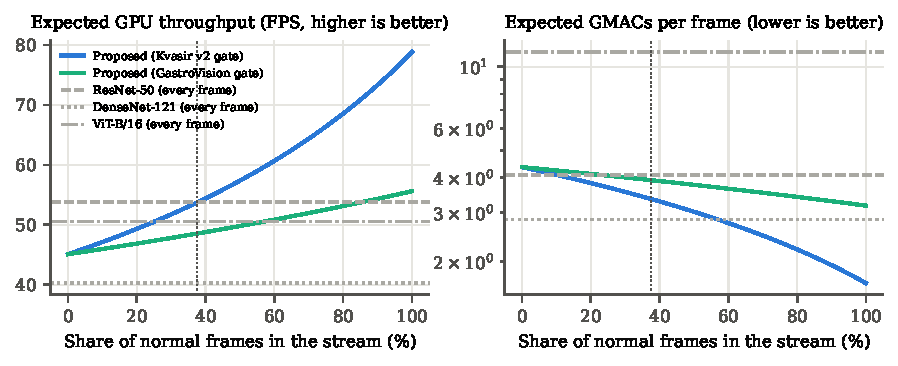
\includegraphics[width=\textwidth]{fig_prevalence.pdf}
\caption{Expected cascade cost as a function of the share of normal frames, computed from the measured component
latencies and the gate's measured recall/specificity: GPU throughput (left) and GMACs per frame (right, log scale).
Grey lines are single-frame baselines run on every frame; the dotted line marks Kvasir's test prevalence.}
\label{fig:prevalence}
\end{figure*}

\begin{figure}[t]
\centering
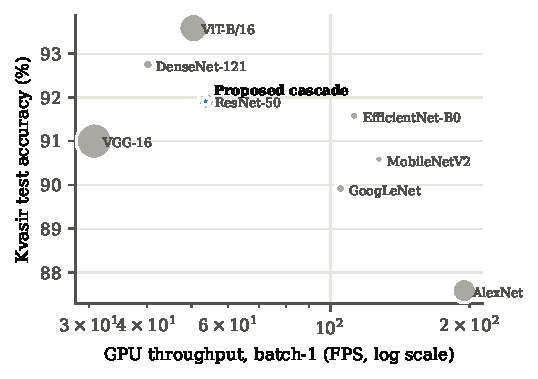
\includegraphics[width=\linewidth]{fig_accuracy_vs_fps.pdf}
\caption{Accuracy versus batch-1 GPU throughput on Kvasir v2 (marker area $\propto$ parameters).}
\label{fig:tradeoff}
\end{figure}

\subsection{Cross-Database Generalisation}
Table~\ref{tab:cross} applies the Kvasir-trained models, without any re-training, to the two pixel-annotated polyp
databases. Kvasir-SEG images are drawn from the same source as Kvasir, so its numbers mainly measure in-domain
consistency; \Rkvasirsegn\ of \Rkvasirsegntotal\ images remain after removing near-duplicates of training images.
CVC-ClinicDB comes from a different hospital and endoscope and is therefore a true domain-shift test. On CVC-ClinicDB
the proposed cascade flags \Rcvcprop\% of the polyp frames as abnormal (\Rcvcproppolyp\% as \emph{polyp}). The
gap between the polyp-class and abnormal-class sensitivities shows that many shifted-domain polyps are still routed to
the lesion branch even when the fine-grained label is wrong, which is the clinically relevant behaviour for a
detection aid. ViT-B/16 and EfficientNet-B0 transfer best to the new domain, which suggests that the Stage-2
backbone, rather than the temporal design, limits cross-domain robustness; on the in-domain Kvasir-SEG images the
proposed cascade has the highest polyp sensitivity (\Rkvasirsegproppolyp\%).

\maybeinput{tables/crossdata}

\subsection{Explainability}
Grad-CAM maps of the Stage-2 network (Fig.~\ref{fig:gradcam}) are compared quantitatively with the expert polyp
masks in Table~\ref{tab:gradcam}. The pointing-game hit rate of the proposed Stage-2 network is \Rgckvasirsegpg\% on
Kvasir-SEG and \Rgccvcpg\% on CVC-ClinicDB, against a random-pointing baseline equal to the mean mask area
(\Rgckvasirsegarea\% and \Rgccvcarea\%). This indicates that the network attends to the lesion itself rather than to
dataset artifacts such as the green position-indicator box or text overlays. Interestingly, the cross-entropy ResNet-50
localises slightly better than the focal-loss version on both databases: focal loss down-weights easy, confidently
classified polyps, which yields lower-confidence and somewhat more diffuse maps; this trade-off between rare-class
sensitivity and map sharpness is worth further study. Finally, the t-SNE embedding
\cite{vandermaaten2008tsne} of the Stage-2 features (Fig.~\ref{fig:tsne}) shows compact class clusters, with the
expected overlap between oesophagitis and Z-line and between the two dyed classes.

\maybeinput{tables/gradcam}

\begin{figure*}[t]
\centering
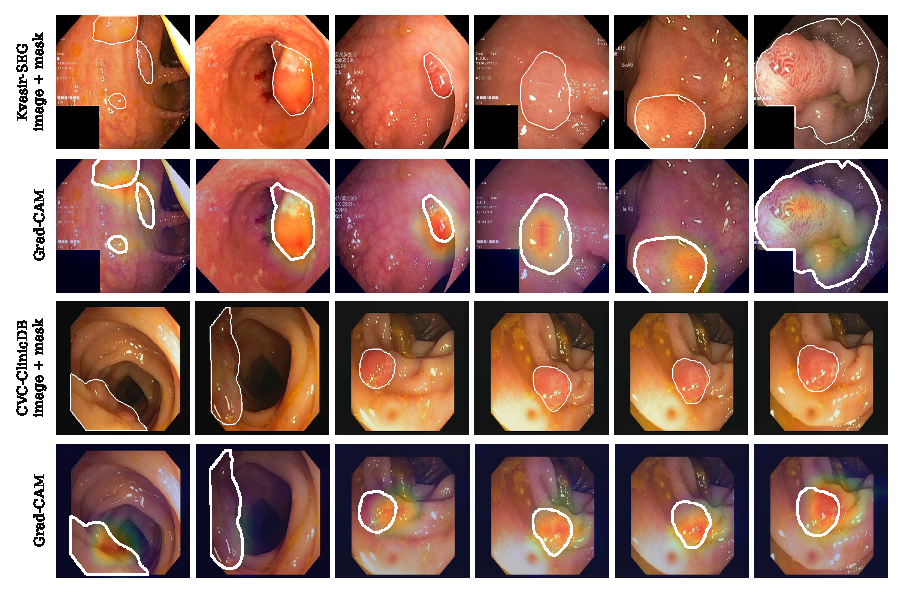
\includegraphics[width=\textwidth]{fig_gradcam.pdf}
\caption{Grad-CAM of the proposed Stage-2 network for the \emph{polyp} class on unseen Kvasir-SEG and CVC-ClinicDB
frames; the expert polyp mask is outlined in white. The map is scaled by the model's confidence.}
\label{fig:gradcam}
\end{figure*}

\begin{figure}[t]
\centering
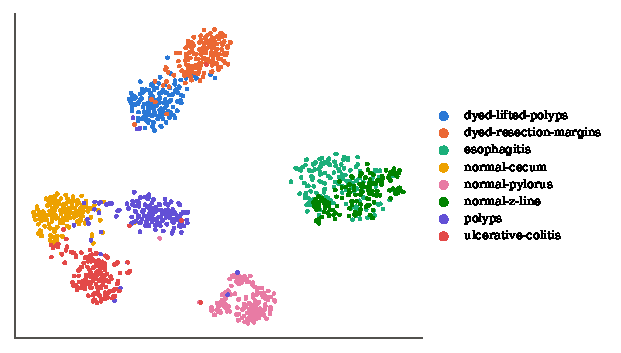
\includegraphics[width=\linewidth]{fig_tsne.pdf}
\caption{t-SNE of the 2048-d Stage-2 features of the Kvasir test images.}
\label{fig:tsne}
\end{figure}

\subsection{Limitations}
The temporal clips are synthesised from still images, so the study measures robustness to \emph{simulated}
artifacts; evaluating on real annotated video (e.g.\ the HyperKvasir video collection \cite{borgli2020hyperkvasir}) is the most important next step.
All networks were fine-tuned for a short, fixed budget on a single train/validation/test split; repeated runs with
different seeds would provide confidence intervals. Rare classes with fewer than 30 images, including gastric
ulcers in GastroVision, had to be excluded, which also limits the strength of the claims for rare gastric
pathologies.


% =====================================================================
\section{Conclusion}
\label{sec:conclusion}
This paper presented a cascaded spatio-temporal framework for GI abnormality detection in endoscopy that combines a
MobileNetV2 gate, a ResNet-50 feature extractor and a Bi-LSTM with temporal attention, trained with focal loss and
explained with Grad-CAM. It was benchmarked against a classical SIFT-BoVW+SVM pipeline and eight deep baselines on
four public databases with classification, efficiency and explainability evaluators. On clean still images the
proposed system comes within \Rgapbest\ points of the best single-frame network (\Rpropacc\% accuracy and \Rpropmcc\%
MCC on Kvasir v2, versus \Rbestbaseacc\% for \Rbestbase). Its
advantage appears when frames are degraded: under transient motion blur, defocus, specular flashes or occlusion it
keeps \Rrobtransient\% accuracy, whereas single-frame baselines fall to \Rrobbestbaseacc\% or less. A temporally
smoothed gate retains $\ge$99\% of abnormal frames while skipping the expensive stages for normal ones, which cuts
the average compute per frame and pays off increasingly as the share of normal frames grows, as in real examinations. Future work will
validate the system on real endoscopic video, add repeated-seed confidence intervals, and extend the label set to
rare gastric pathologies such as early gastric cancer and ulcers.


% =====================================================================
\begin{thebibliography}{40}

\bibitem{pogorelov2017kvasir}
K. Pogorelov et al., ``KVASIR: A Multi-Class Image Dataset for Computer Aided Gastrointestinal Disease Detection,'' in \emph{Proc. 8th ACM Multimedia Systems Conference}, 2017, pp. 164--169.

\bibitem{borgli2020hyperkvasir}
H. Borgli et al., ``HyperKvasir, a comprehensive multi-class image and video dataset for gastrointestinal endoscopy,'' \emph{Scientific Data}, vol. 7, no. 1, p. 283, 2020.

\bibitem{jha2023gastrovision}
D. Jha et al., ``GastroVision: A Multi-class Endoscopy Image Dataset for Computer Aided Gastrointestinal Disease Detection,'' in \emph{ICML Workshop on Machine Learning for Multimodal Healthcare Data}, 2023.

\bibitem{jha2020kvasirseg}
D. Jha et al., ``Kvasir-SEG: A Segmented Polyp Dataset,'' in \emph{Proc. Int. Conf. on Multimedia Modeling (MMM)}, 2020, pp. 451--462.

\bibitem{bernal2015cvc}
J. Bernal et al., ``WM-DOVA maps for accurate polyp highlighting in colonoscopy: Validation vs. saliency maps from physicians,'' \emph{Computerized Medical Imaging and Graphics}, vol. 43, pp. 99--111, 2015.

\bibitem{frontiers2026}
X. Wang et al., ``Deep learning for detecting early gastric cancer with white-light endoscopy: a systematic review and meta-analysis,'' \emph{Frontiers in Artificial Intelligence}, Jan. 2026.

\bibitem{wjg2025}
Y. Chen et al., ``Application of deep learning-based convolutional neural networks in gastrointestinal disease endoscopic examination,'' \emph{World Journal of Gastroenterology}, vol. 31, no. 36, Sep. 2025.

\bibitem{lowe2004sift}
D. G. Lowe, ``Distinctive Image Features from Scale-Invariant Keypoints,'' \emph{International Journal of Computer Vision}, vol. 60, no. 2, pp. 91--110, 2004.

\bibitem{csurka2004bovw}
G. Csurka, C. Dance, L. Fan, J. Willamowski, and C. Bray, ``Visual categorization with bags of keypoints,'' in \emph{ECCV Workshop on Statistical Learning in Computer Vision}, 2004.

\bibitem{ojala2002lbp}
T. Ojala, M. Pietik{\"a}inen, and T. M{\"a}enp{\"a}{\"a}, ``Multiresolution gray-scale and rotation invariant texture classification with local binary patterns,'' \emph{IEEE Trans. Pattern Analysis and Machine Intelligence}, vol. 24, no. 7, pp. 971--987, 2002.

\bibitem{cortes1995svm}
C. Cortes and V. Vapnik, ``Support-vector networks,'' \emph{Machine Learning}, vol. 20, no. 3, pp. 273--297, 1995.

\bibitem{krizhevsky2012imagenet}
A. Krizhevsky, I. Sutskever, and G. E. Hinton, ``ImageNet classification with deep convolutional neural networks,'' \emph{Advances in Neural Information Processing Systems}, vol. 25, 2012.

\bibitem{simonyan2014very}
K. Simonyan and A. Zisserman, ``Very Deep Convolutional Networks for Large-Scale Image Recognition,'' in \emph{International Conference on Learning Representations (ICLR)}, 2015.

\bibitem{szegedy2015going}
C. Szegedy et al., ``Going Deeper with Convolutions,'' in \emph{Proc. IEEE Conf. Computer Vision and Pattern Recognition (CVPR)}, 2015, pp. 1--9.

\bibitem{szegedy2016rethinking}
C. Szegedy et al., ``Rethinking the Inception Architecture for Computer Vision,'' in \emph{Proc. IEEE Conf. Computer Vision and Pattern Recognition (CVPR)}, 2016, pp. 2818--2826.

\bibitem{he2016deep}
K. He, X. Zhang, S. Ren, and J. Sun, ``Deep Residual Learning for Image Recognition,'' in \emph{Proc. IEEE Conf. Computer Vision and Pattern Recognition (CVPR)}, 2016, pp. 770--778.

\bibitem{huang2017densely}
G. Huang, Z. Liu, L. Van Der Maaten, and K. Q. Weinberger, ``Densely Connected Convolutional Networks,'' in \emph{Proc. IEEE Conf. Computer Vision and Pattern Recognition (CVPR)}, 2017, pp. 4700--4708.

\bibitem{mdpi2023sensors}
M. U. Rahman et al., ``Endoscopic Image Classification Based on Explainable Deep Learning,'' \emph{Sensors}, vol. 23, no. 6, p. 3176, 2023.

\bibitem{selvaraju2017grad}
R. R. Selvaraju et al., ``Grad-CAM: Visual Explanations from Deep Networks via Gradient-Based Localization,'' in \emph{Proc. IEEE Int. Conf. Computer Vision (ICCV)}, 2017, pp. 618--626.

\bibitem{ronneberger2015u}
O. Ronneberger, P. Fischer, and T. Brox, ``U-Net: Convolutional Networks for Biomedical Image Segmentation,'' in \emph{Medical Image Computing and Computer-Assisted Intervention (MICCAI)}, 2015, pp. 234--241.

\bibitem{ren2015faster}
S. Ren, K. He, R. Girshick, and J. Sun, ``Faster R-CNN: Towards Real-Time Object Detection with Region Proposal Networks,'' \emph{Advances in Neural Information Processing Systems}, vol. 28, 2015.

\bibitem{he2017mask}
K. He, G. Gkioxari, P. Doll{\'a}r, and R. Girshick, ``Mask R-CNN,'' in \emph{Proc. IEEE Int. Conf. Computer Vision (ICCV)}, 2017, pp. 2961--2969.

\bibitem{sandler2018mobilenetv2}
M. Sandler, A. Howard, M. Zhu, A. Zhmoginov, and L.-C. Chen, ``MobileNetV2: Inverted Residuals and Linear Bottlenecks,'' in \emph{Proc. IEEE Conf. Computer Vision and Pattern Recognition (CVPR)}, 2018, pp. 4510--4520.

\bibitem{tan2019efficientnet}
M. Tan and Q. Le, ``EfficientNet: Rethinking Model Scaling for Convolutional Neural Networks,'' in \emph{International Conference on Machine Learning (ICML)}, 2019, pp. 6105--6114.

\bibitem{mdpi2024ensemble}
A. Ahmed et al., ``Gastrointestinal Lesion Detection Using Ensemble Deep Learning Through Global Contextual Information,'' \emph{Bioengineering}, vol. 12, no. 1, 2024.

\bibitem{bochkovskiy2020yolov4}
A. Bochkovskiy, C. Y. Wang, and H. Y. M. Liao, ``YOLOv4: Optimal Speed and Accuracy of Object Detection,'' \emph{arXiv preprint arXiv:2004.10934}, 2020.

\bibitem{kingma2014adam}
D. P. Kingma and J. Ba, ``Adam: A Method for Stochastic Optimization,'' in \emph{International Conference on Learning Representations (ICLR)}, 2015.

\bibitem{loshchilov2019adamw}
I. Loshchilov and F. Hutter, ``Decoupled Weight Decay Regularization,'' in \emph{International Conference on Learning Representations (ICLR)}, 2019.

\bibitem{loshchilov2017sgdr}
I. Loshchilov and F. Hutter, ``SGDR: Stochastic Gradient Descent with Warm Restarts,'' in \emph{International Conference on Learning Representations (ICLR)}, 2017.

\bibitem{lin2017focal}
T.-Y. Lin, P. Goyal, R. Girshick, K. He, and P. Doll{\'a}r, ``Focal Loss for Dense Object Detection,'' in \emph{Proc. IEEE Int. Conf. Computer Vision (ICCV)}, 2017, pp. 2980--2988.

\bibitem{dosovitskiy2020image}
A. Dosovitskiy et al., ``An Image is Worth 16x16 Words: Transformers for Image Recognition at Scale,'' in \emph{International Conference on Learning Representations (ICLR)}, 2021.

\bibitem{hochreiter1997lstm}
S. Hochreiter and J. Schmidhuber, ``Long Short-Term Memory,'' \emph{Neural Computation}, vol. 9, no. 8, pp. 1735--1780, 1997.

\bibitem{schuster1997bidirectional}
M. Schuster and K. K. Paliwal, ``Bidirectional recurrent neural networks,'' \emph{IEEE Trans. Signal Processing}, vol. 45, no. 11, pp. 2673--2681, 1997.

\bibitem{chicco2020mcc}
D. Chicco and G. Jurman, ``The advantages of the Matthews correlation coefficient (MCC) over F1 score and accuracy in binary classification evaluation,'' \emph{BMC Genomics}, vol. 21, no. 6, 2020.

\bibitem{zhang2018pointing}
J. Zhang, S. A. Bargal, Z. Lin, J. Brandt, X. Shen, and S. Sclaroff, ``Top-down Neural Attention by Excitation Backprop,'' \emph{International Journal of Computer Vision}, vol. 126, pp. 1084--1102, 2018.

\bibitem{vandermaaten2008tsne}
L. van der Maaten and G. Hinton, ``Visualizing Data using t-SNE,'' \emph{Journal of Machine Learning Research}, vol. 9, pp. 2579--2605, 2008.

\end{thebibliography}

\end{document}
